\documentclass{beamer}

%%%%%%%%%%%%%%%%%%%%%%%%%%%%%%%%%%
% PAKCAGES
%%%%%%%%%%%%%%%%%%%%%%%%%%%%%%%%%%

\usepackage{etoolbox}
\usepackage{xparse}
\usepackage{graphicx}
\usepackage{subcaption}
\usepackage{moresize}
\usepackage{anyfontsize}
\usepackage{bm} %use bold in math
\usepackage[utf8]{inputenc}
\usepackage[english]{babel}
\usepackage{xcolor}
\usepackage{cancel} % use xcancel see https://jansoehlke.com/2010/06/strikethrough-in-latex/
\usepackage{changepage} % https://tex.stackexchange.com/a/160827/145331
\usepackage{makecell} % https://tex.stackexchange.com/a/11694/145331
\usepackage{multirow}

\usepackage{tikz}
\usetikzlibrary{matrix}
\usetikzlibrary{arrows,automata}
\tikzset{square matrix/.style={
        matrix of nodes,
        column sep=-\pgflinewidth, row sep=-\pgflinewidth,
        nodes={
            draw,
            minimum height=30pt,
            minimum width=30pt,
            anchor=center,
            text width=#1,
            align=center,
            inner sep=0pt
        },
    },
    square matrix/.default=0.6cm
}

\usepackage{calculator}



\makeatletter

% add input source files
% set the input path.
% EXAMPLE \setInputPath{{src/images}{src/tikzs}}
\NewDocumentCommand{\setInputPath}{m}{%
    \def\input@path{#1}%
}

\NewDocumentCommand{\setFontSize}{m o m}{%
    \IfNoValueF{#2}{%
        \fontsize{#1}{#2}\selectfont#3%
    }{%
        % see https://texblog.org/2012/08/29/changing-the-font-size-in-latex/
        \MULTIPLY{#1}{1.2}{\setFont@baseline}%
        \fontsize{#1}{\setFont@baseline}\selectfont#3%
    }%
}

\makeatother
\NewDocumentCommand{\CPD}{}{%
    \texttt{CPD}%
}

\NewDocumentCommand{\ALT}{}{%
    \texttt{ALT}%
}

\NewDocumentCommand{\AWA}{}{%
    \texttt{AWA$^*$}%
}

\NewDocumentCommand{\WA}{}{%
    \texttt{WA$^*$}%
}

\NewDocumentCommand{\A}{}{%
    \texttt{A$^*$}%
}

\NewDocumentCommand{\CPDSearch}{}{%
    \texttt{CPD-Search}%
}

\NewDocumentCommand{\anytimeCPDSearch}{}{%
    \texttt{Anytime CPD-Search}%
}


\NewDocumentCommand{\CPDPathName}{}{%
    \texttt{CPD}-Path%
}

\NewDocumentCommand{\CPDPathsName}{}{%
    \texttt{CPD}-Paths%
}

\NewDocumentCommand{\CPDPath}{m m}{%
    \texttt{CPD-Path}[#1, #2]%
}

\NewDocumentCommand{\CPDPathCostOriginal}{m m}{%
    \ifmmode{h_{CPD}[#1]}\else{$h_{CPD}[#1]$}\fi%
}

\NewDocumentCommand{\CPDPathCostNew}{m m}{%
    \ifmmode{h'_{CPD}[#1]}\else{$h'_{CPD}[#1]$}\fi%
}

\NewDocumentCommand{\pathOnGraph}{m m}{%
    path[#1, #2]%
}

%%%%%%%%%%%%%%%%%%%%%%%%%%%%%%%%%%%%%%%
% CONFIGURATIONS
%%%%%%%%%%%%%%%%%%%%%%%%%%%%%%%%%%%%%%%

%beamer theme
\usetheme{Frankfurt}

\setbeamertemplate{itemize item}{$\bm{\diamond}$}
\setbeamertemplate{itemize subitem}{$\bm{-}$}

\title{Path Planning with CPD Heuristics}
\author{Massimo Bono$^1$, Alfonso E. Gerevini$^1$, Daniel D. Harabor$^2$ and Peter J.Stuckey$^2$}
\institute{%
    $^1$\setFontSize{7.8}{Dipartimento di Ingegneria dell'Informazione, Università degli Studi di Brescia, Italy}%
    \\%
    $^2$\setFontSize{7.8}{Faculty of Information Technology, Monash University, Melbourne, Australia}%
    \\%
    \{mbono, alfonso.gerevini\}@unibs.it, \{daniel.harabor, peter.stuckey\}@monash.edu%
}
%\date{\today}
\date{August 15, 2019}

\newcommand{\addToInputPath}[1]{%
    \makeatletter
    \providecommand*{\input@path}{}
    \g@addto@macro\input@path{#1}% append
    \input@path
    \makeatother
}

% \addToInputPath{%
%     {src/texs}%
%     {src/images}%
%     {src/tikzs}%
%     {src/bibs}%
% }

%%%%%%%%%%%%%%%%%%%%%%%%%%%%%%%%%%%%%%%%%%%%
% DOCUMENT
%%%%%%%%%%%%%%%%%%%%%%%%%%%%%%%%%%%%%%%%%%%%

\begin{document}

%https://stackoverflow.com/a/3210406/1887602
\beamertemplatenavigationsymbolsempty

% tempo totale: 13 minuti => 50 secondi per slide! è chiaro che qualche slide va rimossa
% High level
% SLIDE 1: titolo
% SLIDE 2: 
%    - path finding è importante (videogiochi, routing); moderne soluzioni usano auxiliary data per calcolare velocemente;
%    - una variante del problema è quella in cui i costi degli archi non sono fissi, ma cambiano. 
%    - data una mappa, dopo che delle perturbazioni non decrescenti l'hanno modificata, come possiamo calcolare velocemente il percorso ottimo?
%    - quest apresentazione cercherà di rispondere a questa domanda.
% SLIDE 3: 
%   - esempio per motivare il lavoro: siamo su una mappa stradale e stiamo seguendo un percorso ottimo. Ad un certo punto
% sul nostro percorso ottimo scopriamo che  c'è un ingorgo che ci rallenterebbe. Abbiamo quindi la scelta di:
% ricalcolare il nostro percorso ottimo da zero sulla nuova mappa (mappa originale + perturbazioni) oppure possiamo
% cercare di calcolare il percorso ottimo sfruttando le informazioni precedenti (mappa originale senza perturbazioni)
% SLIDE 4: table of contents
%   context and background: CPD, ALT, AWA*
%   proposed technique:
%       - CPD Search
%       - Anytime CPD Search
%   Experimental results:
%       - optimal;
%       - anytime;
%   Conclusions and future works;
% SLIDE 5: secondo me qui è meglio scrivere bene il nostro context (ovvero perturbazioni online, preprocessing offline) dato
%   che è stato un punto che ha creato criticità nella rebuttal;
%   - il tempo di prerocessing offline non deve essere ammortizzato nell'online;
% SLIDE 6: CPD (citazione)
%   - esempio di costruzione (per intenderci quello con la mappa 3x3, non quello di Harabor nel paper);
%   - esempio di matrice delle adiacenze => compressione con un mini esempio;
%   - esempio di query, come si fa inserendo la complessità (da s -> a, da a->b, da b -> g);
% SLIDE 7: ALT (citazione)
%   - disuguaglianza triangolare con il massimo;
%   - Dico come abbiamo fatto a posizionare i landmark;
% SLIDE 8: AWA* (citazione)
%   - Idea: usare le soluzione trovate per fare pruning sulla ricerca;
% SLIDE 9: CPD-Search
%   - nodo di ricerca: location
%   - MAIN IDEAS:
%       * il percorso calcolato dal CPD nella mappa originale è un lowerbound del percorso ottimo calcolabile
%       nella mappa parturbata (siccome le perturbazioni sono non-decrescenti) => euristica ammissibile;
%       * dato una posizione s, se il percorso generato dal CPD (che è ottimo) è privo di perturbazioni possiamo terminare la ricerca e calcolare
%           immediatamente il percorso ottimo => early termination;
% SLIDE 10: sicuramente qui andrebbe messo qualcosa in più della "main idea". Il problema è che non voglio mettere l'algoritmo... troppo
% lungo e complesso da commmentare.
% SLIDE 11: Experimental setup
%   - map pool: Sturtevant;
%   - how we generated perturbations:
%       - random perturbations on 10% of edges of the map (3x the original cost);
%       - perturbation affecting a whole area on a location on the optimal path of a query (up to 4x the original cost);
% SLIDE 12:
%   - optimal search:
%       - results on the cactus plots (hrt201n, dustwallowkeys, mazes);
% SLIDE 13
%   - anytime search:
%       - results on hrt201n map;
% SLIDE 14: Conclusion and Future works
%   - we applied CPD technique in the context of dynamic edge-cost;
%   - we proposed the application in the optimal, bounded and anytime context;
%   - we have experimentally evaluated the techniques performances against ALT's and showed significant gains;
%   FUTURE WORKS:
%   - application of CPD over temporally changing edge-costs for deisgning admissible and unadmissible heuristics;
%   - application of CPD in the MAPF setting;
%   - dare l'idea sulle idee di harabor /idee di saetti?
%       
%          



\begin{frame}[plain]
    \titlepage
    %TODO add brescia and monash logos
    \begin{minipage}{0.5\textwidth}
        \begin{figure}
            \centering
            \includegraphics[width=0.8\textwidth]{src/images/monash}
        \end{figure}
    \end{minipage}\hfill%
    \begin{minipage}{0.5\textwidth}
        \begin{figure}
            \centering
            \includegraphics[width=0.8\textwidth]{src/images/unibs}
        \end{figure}
    \end{minipage}%
\end{frame}
\section*{Introduction}

\begin{frame}{Introduction}
    \begin{itemize}
        \item Single-agent shortest path planning: given a graph, compute a path from a start node $s$ to a goal $t$ whose cost is minimum;
        \item Modern algorithms use auxiliary data structures to improve performances;
        \item However, when \textbf{edge costs are dynamic} such algorithms may fail due to invalid auxiliary data.
        
        \medskip

        \item \textbf{Goal}: Solve dynamic-cost single agent path planning problems by exploiting Compressed Path Database (CPD);
        \item \textbf{Results}: new bounded A* variant using CPD whose experimentally-evaluated performances show substantial gains over previous algorithms.
    \end{itemize}
\end{frame}

% see https://tex.stackexchange.com/a/208409/145331
\begin{frame}[fragile]{A simple example}

    \only<1>{
        \begin{center}
            \textbf{Original Map}

            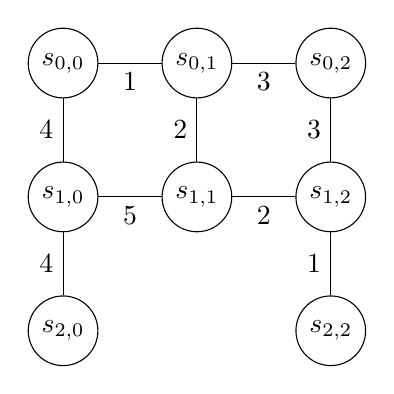
\begin{tikzpicture}
                \tikzset{Vertex/.style={%
                    shape=circle,%
                    draw=black,%
                    minimum size=10pt,%
                    radius=1cm,%
                    inner sep=3pt,%
                    node distance=1.7cm,%
                }}
        
                \node[Vertex] (v00) at (0,0) {$s_{0,0}$};
                \node[Vertex, right of=v00] (v01) {$s_{0,1}$};
                \node[Vertex, right of=v01] (v02) {$s_{0,2}$};
                \node[Vertex, below of=v00] (v10) {$s_{1,0}$};
                \node[Vertex, right of=v10] (v11) {$s_{1,1}$};
                \node[Vertex, right of=v11] (v12) {$s_{1,2}$};
                \node[Vertex, below of=v10] (v20) {$s_{2,0}$};
                \node[Vertex, below of=v12] (v22) {$s_{2,2}$};
        
                \path (v00) edge[-.] node[below]{1} (v01);
                \path (v01) edge[-.] node[below]{3} (v02);
                \path (v10) edge[-.] node[below]{5} (v11);
                \path (v11) edge[-.] node[below]{2} (v12);
                \path (v00) edge[-.] node[left]{4} (v10);
                \path (v10) edge[-.] node[left]{4} (v20);
                \path (v01) edge[-.] node[left]{2} (v11);
                \path (v02) edge[-.] node[left]{3} (v12);
                \path (v12) edge[-.] node[left]{1} (v22);
            \end{tikzpicture}
        \end{center}
    }%
    \only<2>{
        \begin{center}
            \textbf{Original Map}

            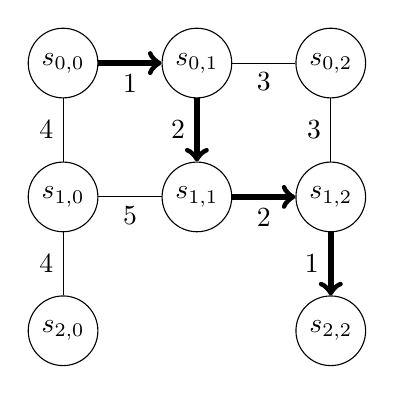
\begin{tikzpicture}
                \tikzset{Vertex/.style={%
                    shape=circle,%
                    draw=black,%
                    minimum size=10pt,%
                    radius=1cm,%
                    inner sep=3pt,%
                    node distance=1.7cm,%
                }}
        
                \node[Vertex] (v00) at (0,0) {$s_{0,0}$};
                \node[Vertex, right of=v00] (v01) {$s_{0,1}$};
                \node[Vertex, right of=v01] (v02) {$s_{0,2}$};
                \node[Vertex, below of=v00] (v10) {$s_{1,0}$};
                \node[Vertex, right of=v10] (v11) {$s_{1,1}$};
                \node[Vertex, right of=v11] (v12) {$s_{1,2}$};
                \node[Vertex, below of=v10] (v20) {$s_{2,0}$};
                \node[Vertex, below of=v12] (v22) {$s_{2,2}$};
        
                \path (v00) edge[->,line width=2pt] node[below]{1} (v01);
                \path (v01) edge[-.] node[below]{3} (v02);
                \path (v10) edge[-.] node[below]{5} (v11);
                \path (v11) edge[->,line width=2pt] node[below]{2} (v12);
                \path (v00) edge[-.] node[left]{4} (v10);
                \path (v10) edge[-.] node[left]{4} (v20);
                \path (v01) edge[->,line width=2pt] node[left]{2} (v11);
                \path (v02) edge[-.] node[left]{3} (v12);
                \path (v12) edge[->,line width=2pt] node[left]{1} (v22);
            \end{tikzpicture}

            $$s_{0,0} \rightarrow s_{0,1} \rightarrow s_{1,1} \rightarrow s_{1,2} \rightarrow s_{2,2}$$
        \end{center}
    }%
    \only<3>{
        \begin{center}
            \textbf{Perturbated Map}

            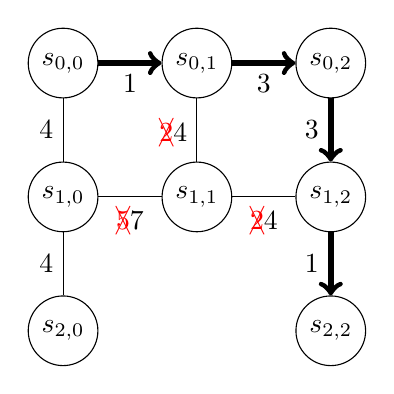
\begin{tikzpicture}
                \tikzset{Vertex/.style={%
                    shape=circle,%
                    draw=black,%
                    minimum size=10pt,%
                    radius=1cm,%
                    inner sep=3pt,%
                    node distance=1.7cm,%
                }}
        
                \node[Vertex] (v00) at (0,0) {$s_{0,0}$};
                \node[Vertex, right of=v00] (v01) {$s_{0,1}$};
                \node[Vertex, right of=v01] (v02) {$s_{0,2}$};
                \node[Vertex, below of=v00] (v10) {$s_{1,0}$};
                \node[Vertex, right of=v10] (v11) {$s_{1,1}$};
                \node[Vertex, right of=v11] (v12) {$s_{1,2}$};
                \node[Vertex, below of=v10] (v20) {$s_{2,0}$};
                \node[Vertex, below of=v12] (v22) {$s_{2,2}$};
        
                \path (v00) edge[->,line width=2pt] node[below]{1} (v01);
                \path (v01) edge[->,line width=2pt] node[below]{3} (v02);
                \path (v10) edge[-.] node[below]{{\color{red} \xcancel{5}}{7}} (v11);
                \path (v11) edge[-.] node[below]{{\color{red} \xcancel{2}}{4}} (v12);
                \path (v00) edge[-.] node[left]{4} (v10);
                \path (v10) edge[-.] node[left]{4} (v20);
                \path (v01) edge[-.] node[left]{{\color{red} \xcancel{2}}{4}} (v11);
                \path (v02) edge[->,line width=2pt] node[left]{3} (v12);
                \path (v12) edge[->,line width=2pt] node[left]{1} (v22);
            \end{tikzpicture}

            $$s_{0,0} \rightarrow s_{0,1} \rightarrow s_{0,2} \rightarrow s_{1,2} \rightarrow s_{2,2}$$
        \end{center}
    }
    
\end{frame}


% \begin{frame}[fragile]{A simple example}
%     \begin{center}
%         \textbf{Original Map}\\
%     \end{center}

%     \begin{minipage}{0.5\textwidth}
%         \begin{tikzpicture}
%             \matrix[square matrix]{
%                 |[fill=black!0]| $s_{0,0}$   &|[fill=black!0]| $s_{0,1}$  &|[fill=black!40]| $s_{0,2}$  \\
%                 |[fill=black!60]| $s_{1,0}$   &|[fill=black!20]| $s_{1,1}$  &|[fill=black!0]| $s_{1,2}$  \\
%                 |[fill=black!0]| $s_{2,0}$   &|[fill=black]|  &|[fill=black!0]| $s_{2,2}$  \\
%             };
%         \end{tikzpicture}
        
%         \begin{tabular}{clcl}
%             \drawFilledSquare{black!0} & 1 &
%             \drawFilledSquare{black!20} & 3 \\
%             \drawFilledSquare{black!40} & 5 &
%             \drawFilledSquare{black!60} & 7 \\
%             \drawFilledSquare{black} & $\infty$ &
%             & \\
%         \end{tabular}
%     \end{minipage}%
%     \begin{minipage}{0.5\textwidth}
%         \begin{tikzpicture}
%             \tikzset{Vertex/.style={%
%                 shape=circle,%
%                 draw=black,%
%                 minimum size=10pt,%
%                 radius=1cm,%
%                 inner sep=3pt,%
%                 node distance=1.7cm,%
%             }}
    
%             \node[Vertex] (v00) at (0,0) {$s_{0,0}$};
%             \node[Vertex, right of=v00] (v01) {$s_{0,1}$};
%             \node[Vertex, right of=v01] (v02) {$s_{0,2}$};
%             \node[Vertex, below of=v00] (v10) {$s_{1,0}$};
%             \node[Vertex, right of=v10] (v11) {$s_{1,1}$};
%             \node[Vertex, right of=v11] (v12) {$s_{1,2}$};
%             \node[Vertex, below of=v10] (v20) {$s_{2,0}$};
%             \node[Vertex, below of=v12] (v22) {$s_{2,2}$};
    
%             \path (v00) edge[-.,line width=2pt] node[below]{1} (v01);
%             \path (v01) edge[-.] node[below]{3} (v02);
%             \path (v10) edge[-.] node[below]{5} (v11);
%             \path (v11) edge[-.,line width=2pt] node[below]{2} (v12);
%             \path (v00) edge[-.] node[left]{4} (v10);
%             \path (v10) edge[-.] node[left]{4} (v20);
%             \path (v01) edge[-.,line width=2pt] node[left]{2} (v11);
%             \path (v02) edge[-.] node[left]{3} (v12);
%             \path (v12) edge[-.,line width=2pt] node[left]{1} (v22);
%         \end{tikzpicture}
%         $$s_{0,0} \rightarrow s_{0,1} \rightarrow s_{1,1} \rightarrow s_{1,2} \rightarrow s_{2,2}$$
%     \end{minipage}
% \end{frame}

% \begin{frame}[fragile]{A simple example}
%     \begin{center}
%         \textbf{Perturbated Map}\\
%     \end{center}

%     \begin{minipage}{0.5\textwidth}
%         \begin{tikzpicture}
%             \matrix[square matrix]{
%                 |[fill=black!0]| $s_{0,0}$   &|[fill=black!0]| $s_{0,1}$  &|[fill=black!40]| $s_{0,2}$  \\
%                 |[fill=black!60]| $s_{1,0}$   &|[fill=black!60]| $s_{1,1}$  &|[fill=black!0]| $s_{1,2}$  \\
%                 |[fill=black!0]| $s_{2,0}$   &|[fill=black]|  &|[fill=black!0]| $s_{2,2}$  \\
%             };
%         \end{tikzpicture}
        
%         \begin{tabular}{clcl}
%             \drawFilledSquare{black!0} & 1 &
%             \drawFilledSquare{black!20} & 3 \\
%             \drawFilledSquare{black!40} & 5 &
%             \drawFilledSquare{black!60} & 7 \\
%             \drawFilledSquare{black} & $\infty$ &
%             & \\
%         \end{tabular}
%     \end{minipage}%
%     \begin{minipage}{0.5\textwidth}
%         \begin{tikzpicture}
%             \tikzset{Vertex/.style={%
%                 shape=circle,%
%                 draw=black,%
%                 minimum size=10pt,%
%                 radius=1cm,%
%                 inner sep=3pt,%
%                 node distance=1.7cm,%
%             }}
    
%             \node[Vertex] (v00) at (0,0) {$s_{0,0}$};
%             \node[Vertex, right of=v00] (v01) {$s_{0,1}$};
%             \node[Vertex, right of=v01] (v02) {$s_{0,2}$};
%             \node[Vertex, below of=v00] (v10) {$s_{1,0}$};
%             \node[Vertex, right of=v10] (v11) {$s_{1,1}$};
%             \node[Vertex, right of=v11] (v12) {$s_{1,2}$};
%             \node[Vertex, below of=v10] (v20) {$s_{2,0}$};
%             \node[Vertex, below of=v12] (v22) {$s_{2,2}$};
    
%             \path (v00) edge[-.,line width=2pt] node[below]{1} (v01);
%             \path (v01) edge[-.,line width=2pt] node[below]{3} (v02);
%             \path (v10) edge[-.] node[below]{{\color{red} \xcancel{5}}{7}} (v11);
%             \path (v11) edge[-.] node[below]{{\color{red} \xcancel{2}}{4}} (v12);
%             \path (v00) edge[-.] node[left]{4} (v10);
%             \path (v10) edge[-.] node[left]{4} (v20);
%             \path (v01) edge[-.] node[left]{{\color{red} \xcancel{2}}{4}} (v11);
%             \path (v02) edge[-.,line width=2pt] node[left]{3} (v12);
%             \path (v12) edge[-.,line width=2pt] node[left]{1} (v22);
%         \end{tikzpicture}
%         $$s_{0,0} \rightarrow s_{0,1} \rightarrow s_{0,2} \rightarrow s_{1,2} \rightarrow s_{2,2}$$
%     \end{minipage}
% \end{frame}

\begin{frame}{Talk Outline}
    \begin{itemize}
        \item Context and Background:
        \begin{itemize}
            \item Compressed Path Database (\CPD{});
            \item \ALT{}, \AWA{};
        \end{itemize}
        \item Proposed Technique: \CPDSearch{};
        \item Experimental Results: 
            \begin{itemize}
                \item optimal and 
                \item anytime scenario;
            \end{itemize}
        \item Conclusion and Future Work.
    \end{itemize}
\end{frame}
\section*{Background}

\begin{frame}{Context}
    \begin{itemize}
        \item Path planning episodes are independent;
        \item each episode has fixed start and target locations;
        \item graph map is known a priori.
    \end{itemize}
    
    \medskip
    Map edge costs changes (\textit{perturbations}):
    \begin{itemize}
        \item[-] distribution over map unknown a priori;
        \item[-] only increase original edge costs (\eg{} routing in road networks, videogames);
        \item[-] detected at the beginning of each path planning episode and then assumed fixed.
    \end{itemize}
\end{frame}

\begin{frame}{Compressed Path Database (\CPD{})}
    \begin{minipage}{0.33\textwidth}
        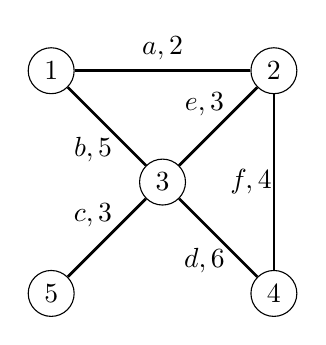
\begin{tikzpicture}
            \tikzset{Vertex/.style={%
                    shape=circle,%
                    draw=black,%
                    minimum size=10pt,%
                    radius=1cm,%
                    inner sep=3pt,%
                    node distance=1.7cm,%
                }}
        
                \node[Vertex] (3) at (0,0) {$3$};
                \node[Vertex] (2) at (+45:2) {$2$};
                \node[Vertex] (1) at (+135:2) {$1$};
                \node[Vertex] (4) at (-45:2) {$4$};
                \node[Vertex] (5) at (-135:2) {$5$};
                
        
                \path (1) edge[-,line width=1pt] node[above]{$a,2$} (2);
                \path (2) edge[-,line width=1pt] node[left,xshift=+3pt]{$f,4$} (4);
                \path (3) edge[-,line width=1pt] node[below,xshift=-5pt]{$b,5$} (1);
                \path (3) edge[-,line width=1pt] node[above,xshift=-5pt]{$e,3$} (2);
                \path (3) edge[-,line width=1pt] node[below,xshift=-5pt]{$d,6$} (4);
                \path (3) edge[-,line width=1pt] node[above,xshift=-5pt]{$c,3$} (5);
        \end{tikzpicture}
    \end{minipage}\hfill%
    \begin{minipage}{0.33\textwidth}
        % see https://tex.stackexchange.com/a/317083/145331
        \begin{table}
            \centering
            \begin{tabular}{l|ccccc}
            \diaghead(5,-3){\theadfont xx}{\hphantom{x}\hphantom{x}t}{s\hphantom{x}\hphantom{x}} 
                & 1 & 2 & 3 & 4 & 5 \\ \hline
                1 & - & $a$ & $a$ & $a$ & $a$ \\
                2 & $a$ & - & $e$ & $f$ & $e$ \\
                3 & $e$ & $e$ & - & $d$ & $c$ \\
                4 & $f$ & $f$ & - & $d$ & $d$ \\
                5 & $c$ & $c$ & $c$ & $c$ & - \\
            \end{tabular}
        \end{table}
    \end{minipage}\hfill%
    \begin{minipage}{0.33\textwidth}
        $$(s,t) = (1, 5)$$
        $$M[1, 5] = a$$
        $$M[2, 5] = e$$
        $$M[3, 5] = c$$
        $$1 \rightarrow 2 \rightarrow 3 \rightarrow 5$$
    \end{minipage}

\end{frame}

\begin{frame}{\ALT{} and Anytime Weighted A* (\AWA{})}
    \textbf{\ALT{}:}
    \begin{itemize}
        \item Search technique using preprocessed \textit{landmarks} to derive admissible
            estimates of node pair $(s, t)$;
    \end{itemize}
    \textbf{\AWA{}:}
    \begin{itemize}
        \item \WA{} anytime variant iteratively computing suboptimal solutions while updating in the tightest possible way the suboptimality bound;
    \end{itemize}
\end{frame}
\section*{Proposed Techniques}

\begin{frame}{\CPDSearch{}}
\end{frame}
\section*{Experiments}

\begin{frame}{Experimental Setup}
\end{frame}

\begin{frame}{Optimal scenario}
\end{frame}

\begin{frame}{Anytime scenario}
\end{frame}
\section*{Conclusions}

\begin{frame}{Conclusions and Future Works}
    \begin{itemize}
        \item Proposed \CPD{}s as heuristic functions for dynamic settings where costs can only increase;
        \medskip
        \item developed a new algorithm, \CPDSearch{} which can be used in both optimal and anytime context;
        \medskip
        \item Experimental analysis performances showing improvements \wrt{} state-of-the-art (\ALT{} and \AWA{});
        \medskip
        \item \textbf{Future Work} includes explore \CPD{} usage in Multi-Agent Path Finding context.
    \end{itemize}
\end{frame}


\end{document}
